\documentclass[11pt,a4paper]{article}
\usepackage[a4paper,hmargin=1in,vmargin=1in]{geometry}
\usepackage{pgfplots}
\pgfplotsset{compat=1.17}

\usepackage[british]{babel}
\usepackage[utf8]{inputenc}
\usepackage[T1]{fontenc}

\usepackage[nodayofweek]{datetime}
\newdate{date}{16}{1}{2024}

\usepackage{stddoc}
\usepackage{subcaption}


\begin{document}

    \pagenumbering{arabic}

    % Header
    \begin{center}
        {\LARGE\textbf{B2M17NKA - Project I}}\\[3mm]
        \begin{minipage}{0.4\textwidth}
            \begin{flushleft}
                \textsc{\displaydate{date}}
            \end{flushleft}
        \end{minipage}
        ~
        \begin{minipage}{0.4\textwidth}
            \begin{flushright}
                \textsc{Martin Šimák}
            \end{flushright}
        \end{minipage}
        \noindent\rule{14.5cm}{0.4pt}
    \end{center}

    \paragraph{Task 1} \emph{Design of a patch antenna using the transmission line model}\\
    Determine the dimensions and characteristics of a rectangular microstrip patch antenna with linear polarization using the \emph{Transmission Line Model} (TLM). An illustration of such antenna can be seen in Figure~\ref{fig:patch-antenna-illustration}.
    \begin{figure}[!ht]
        \centering
        \includegraphics[width=.5\textwidth]{src/patch-antenna-illustration.png}
        \caption{\label{fig:patch-antenna-illustration}Patch antenna illustration}
    \end{figure}

    \begin{enumerate}[label=1.\arabic*]
        \item Determine the width $W$ and length $L$ of the antenna.
        \item Illustrate the frequency dependence of the input impedance $Z_{\mathrm{in}}$ and the reflection coefficient $\Gamma$ of an edge-fed antenna calculated using the TLM.
        \item Calculate the input impedance $Z_{\mathrm{in}}|_{L_1 = 0}$ of an edge-fed antenna and determine the distance $L_{\mathrm{match}}$ of the feeding point from the edge of the radiating patch so that the input impedance is $50\, \Omega$. Illustrate the frequency dependence of the input impedance $Z_{\mathrm{in}}$ and the reflection coefficient $\Gamma$ of a matched antenna.
        \item Determine the impedance bandwidth of $\mathit{VSWR} < 2$ manually by reading the frequency dependence of $Z_{\mathrm{in}}$. Compare this with the value obtained from the analytical formula.
        \item Using the analytical formula, illustrate the bandwidth of $\mathit{VSWR} < 2$ dependence on the substrate thickness $h$ and substrate relative permittivity $\epsilon_{r}$ for common values.
        \item Illustrate the radiation patterns in decibels in both $E$- and $H$- plane using a polar diagram.
    \end{enumerate}

    \paragraph{Task 2} \emph{Measurement of a patch antenna}\\
    Measure the input impedance $Z_{\mathrm{in}}$ (extracted from the reflection) of the supplied antenna for 3 various feed offsets $L_1$ (both edge positions and a position of best match).
    \begin{enumerate}[label=2.\arabic*]
        \item Plot the measured $Z_{\mathrm{in}}$ and $|\Gamma|$ into a frequency plot along with the values obtained from TLM.
        \item Compare the measured and modelled resonant frequencies $f_{\mathrm{res}}$ and the bandwidths of $\mathit{VSWR} < 2$; determine percentage errors.
        \item Discuss the causes of differences between the measured and modelled results. Take into account the simplification of the TLM analysis.
    \end{enumerate}

    % \newpage
    \section{Design of a patch antenna using the transmission line model}
        \paragraph{Specification} The particular substrate assigned was DICLAD ($\epsilon_r = 2.6$, $\tan(\delta) = 0.0022$) of thickness $h = 1.5\, \mathrm{mm}$ and the intended resonant frequency is $f_{\mathrm{res}} = 1.8\, \mathrm{GHz}$. The patch thickness was $t = 35\, \mathrm{\mu m}$.

        \subsection{Antenna dimensions}
        From the assigned parameters, the dimensions of the rectangular microstrip patch antenna can be calculated as
        \begin{align}
            \label{eq:antenna-dimensions}
            W &= \frac{c}{2f_{\mathrm{res}}} \sqrt{\frac{2}{\epsilon_r+1}},
        &
            L &= \frac{c}{2f_{\mathrm{res}}\sqrt{\epsilon_{\mathrm{eff}}}}-\Delta L,
        \end{align}
        where
        \begin{align}
            \epsilon_{\mathrm{eff}} &= \frac{\epsilon_r+1}{2} + \frac{\epsilon_r-1}{2}\(1+\frac{12h}{W}\)^{-\frac12}
        \end{align}
        is the effective relative permittivity of a microstrip line and
        \begin{align}
            \Delta L = 0.412h\frac{\(\epsilon_{\mathrm{eff}}+0.3\)\(\dfrac Wh+0.264\)}{\(\epsilon_{\mathrm{eff}}-0.258\)\(\dfrac Wh+0.813\)}
        \end{align}
        is the practical approximation for the normalized extension of the length.

        \subsection{Frequency dependence of input impedance and reflection}
            The theoretical derivation of input impedance of a microstrip patch antenna stems from its equivalence to two identical radiating slots each which can be represented by a parallel admittance $Y_s$ (with conductance $G$ and susceptance $B$). Assuming that $h/\lambda_0 < 1/10$, the conductance and susceptance of slots of finite width $W$ can be calculated as
            \begin{align}
                G &= \frac{W}{120\lambda_0}\(1 - \frac{(k_0h)^2}{24}\),
            &
                B &= \frac{W}{120\lambda_0}\(1-0.636\ln(k_0h)\).
            \end{align}
            The impedance of each slot is then given by $Z_s = 1/Y_s$. The next step towards calculating the impedance of a microstrip patch antenna is to compute the characteristic impedance of the microstrip-line feed which is given by
            \begin{align}
                Z_c = \begin{cases}
                    \dfrac{60}{\sqrt{\epsilon_{\mathrm{eff}}}}\ln\(\dfrac{8h}{W} + \dfrac{W}{4h}\) & \text{for } \dfrac{W}{h} \leq 1,
                \\
                    120\pi\[\sqrt{\epsilon_{\mathrm{eff}}}\(\dfrac{W}{h}+1.393+0.667\ln\(\dfrac{W}{h}+1.444\)\)\]^{-1} & \text{for } \dfrac{W}{h} < 1.
                \end{cases}
            \end{align}
            These two results can be combined to obtain the final impedances of the radiating slots accounting for the feed:
            \begin{align}
                Z_1 &= Z_c\frac{Z_s + \i Z_c\tan(\beta L_1)}{Z_c + \i Z_s\tan(\beta L_1)},
            &
                Z_2 &= Z_c\frac{Z_s + \i Z_c\tan(\beta L_2)}{Z_c + \i Z_s\tan(\beta L_2)},
            \end{align}
            where $L_1$ is the length of the section of the microstrip line from the feed to the first radiating slot (later referred to as the feed offset from an edge of the radiating patch) and $L2 = L - L1$ is the analogous length for the second slot. Furthermore, the formula above features the coefficient $\beta$ which is given by
            \begin{align}
                \beta &= \frac{2\pi\sqrt{\epsilon_{\mathrm{eff}}}}{\lambda_0}.
            \end{align}
            The impedances $Z_1$ and $Z_2$ can be combined to yield the final input impedance of the microstrip patch antenna
            \begin{align}
                \label{eq:input-impedance}
                Z_{\mathrm{in}} &= \(\dfrac{1}{Z_1}+\dfrac{1}{Z_2}\)^{-1}.
            \end{align}
            The reflection coefficient is then computed via the well-known formula
            \begin{align}
                \label{eq:reflection-coefficient}
                \Gamma &= \frac{Z_{\mathrm{in}}-Z_0}{Z_{\mathrm{in}}+Z_0}.
            \end{align}
            The results are shown in Figure~\ref{fig:edge-fed-antenna}.
            \begin{figure}[!ht]
                \centering
                \includegraphics[width=.8\textwidth]{src/edge-fed-antenna.eps}
                \caption{\label{fig:edge-fed-antenna}Input impedance and reflection coefficient frequency plots of an edge-fed antenna}
            \end{figure}

        \subsection{Antenna matching}
            The value of input impedance of the antenna with the feeding point located at one of the edges of the patch is $Z_{\mathrm{in}} = [160.73-6.93\i]\, \Omega$ which is clearly mismatched. For practical purposes, we demand the input impedance of any load to be as close to $50\, \Omega$ (or other reference line impedance) as possible.

            Furthermore, Equation~\ref{eq:input-impedance} along with the steps leading to it can be also used to plot the dependence of the input impedance on the feed offset from an edge of the patch. This dependence is depicted in Figure~\ref{fig:feed-offset-impedance-plot} which can be utilized for the determination of $L_{\mathrm{match}} = 15.65\, \mathrm{mm}$.%
                \footnote{This value was actually obtained via finding the $\min_{L_1 \in (0, L)}|Z_{\mathrm{in}}(L_1) - 50\, \Omega|$ instead of manual plot-reading.}
            \begin{figure}[!ht]
                \centering
                \includegraphics[width=.7\textwidth]{src/feed-offset-impedance-plot.eps}
                \caption{\label{fig:feed-offset-impedance-plot}Input impedance feed-offset plot at the resonant frequency}
            \end{figure}

            The resulting input impedance and reflection coefficient frequency plots for the optimized feed offset $L_{\mathrm{match}}$ are shown in Figure~\ref{fig:matched-antenna}. The value of input impedance of the matched antenna is $Z_{\mathrm{in}} = [50.04 - 2.16\i\,]\Omega$.
            \begin{figure}[!ht]
                \centering
                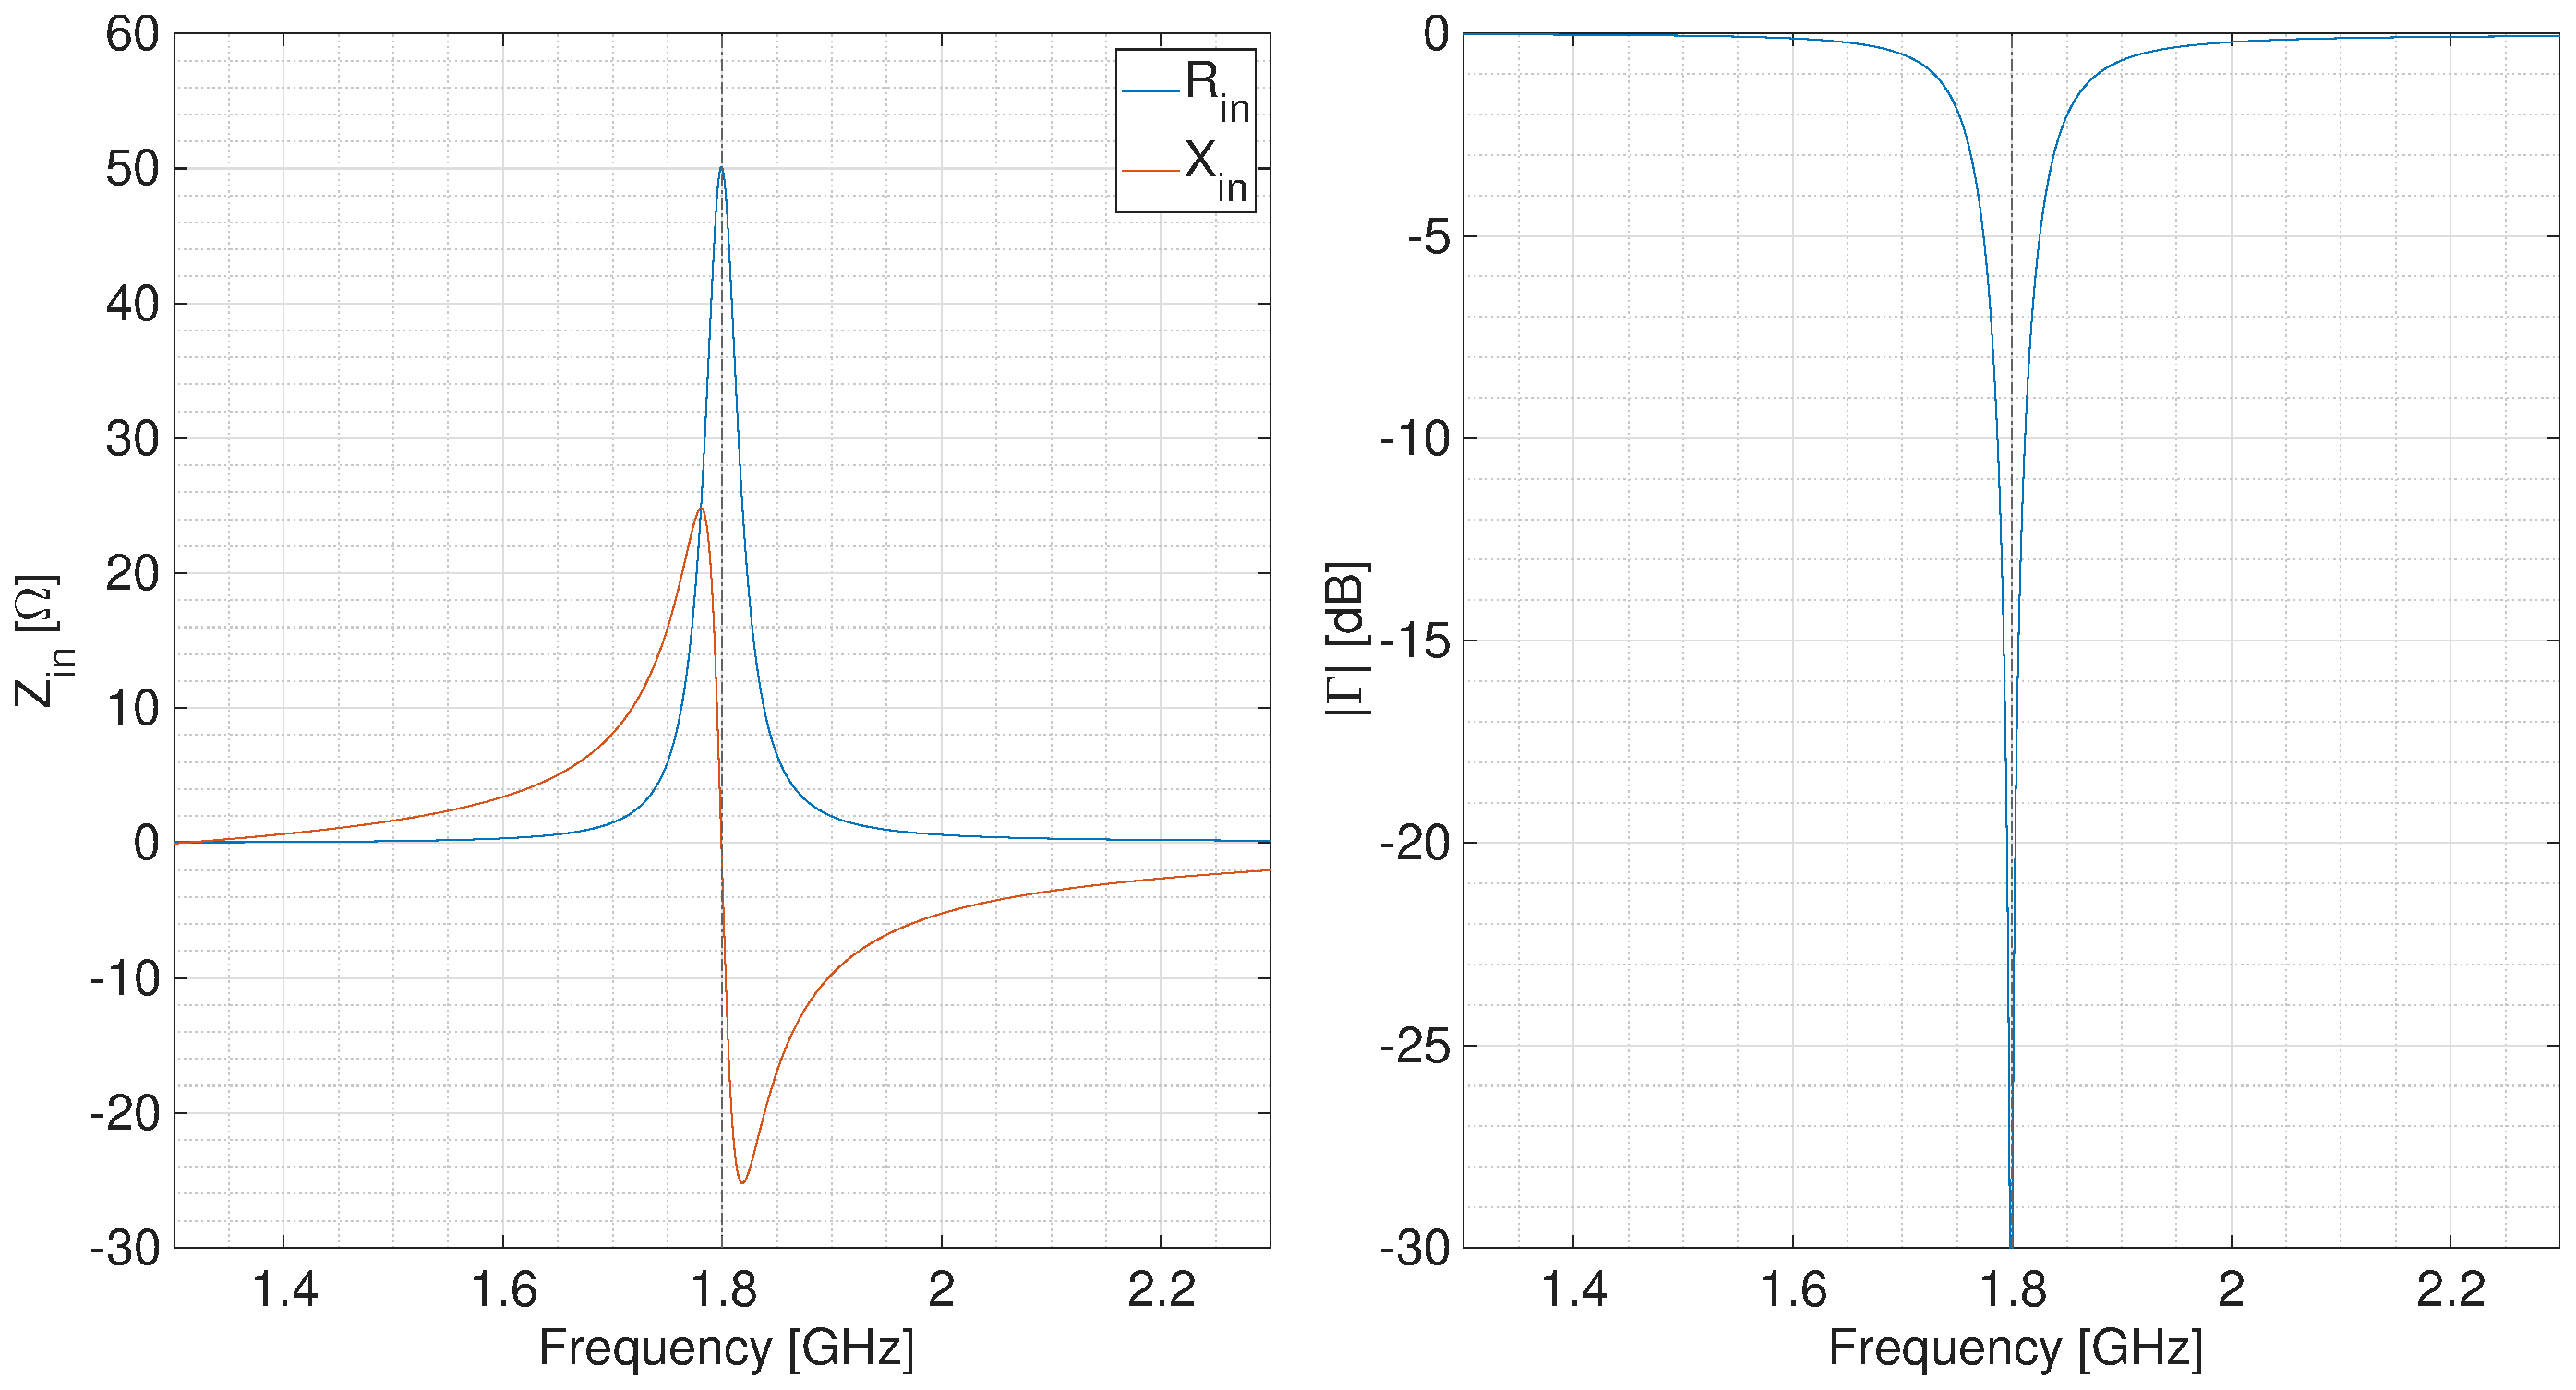
\includegraphics[width=\textwidth]{src/matched-antenna.eps}
                \caption{\label{fig:matched-antenna}Input impedance and reflection coefficient frequency plots of a matched antenna}
            \end{figure}

        \subsection{Impedance bandwidth}
            For the matched antenna, we can determine the frequencies of $|\Gamma(f)| = -9.54\, \mathrm{dB}$ which correspond to the frequencies of $\mathit{VSWR}(f) = 2$. This computed%
                \footnote{$f_{\mathit{VSWR}=2} \in \argmin_{f \in (1.3\, \mathrm{GHz}, 2.3\, \mathrm{GHz})}|\Gamma(f)+9.54\, \mathrm{dB}|$}
            percentage bandwidth yields the value of $\mathit{BW} = 0.02\, \%$ which can be compared to the value obtained from the analytical formula
            \begin{align}
                \label{eq:bandwidth-formula}
                \mathit{BW}(\mathit{VSWR}) &= \frac{\mathit{VSWR}-1}{Q_T \sqrt{\mathit{VSWR}}},
            \end{align}
            where
            \begin{align}
                Q_T = \frac{\omega W_T}{P_d} = \(\frac{1}{Q_d} + \frac{1}{Q_c} + \frac{1}{Q_r}\)^{-1}
            \end{align}
            is the total quality factor consisting of the dielectric quality factor $Q_d$, the conductive quality factor $Q_c$ and the radiation quality factor $Q_r$, each of which corresponds to the respective losses in the structure. Equation~\ref{eq:bandwidth-formula} for $\mathit{VSWR} = 2$ yields the value of $1.75\, \%$ which is slightly different from the one computed using the TLM formulas. This difference can be attributed to the various simplifications introduced during the TLM computations.

        \subsection{Dependence of the impedance bandwidth on substrate properties}
            Using the analytical formula for the bandwidth of $\mathit{VSWR} < 2$ given in Equation~\ref{eq:bandwidth-formula}, we can inspect the dependence of the impedance bandwidth on the substrate properties, namely the substrate height $h$ and its relative permittivity $\epsilon_r$. This dependence is illustrated in Figure~\ref{fig:bandwidth-material-dependence}.
            \begin{figure}[!ht]
                \centering
                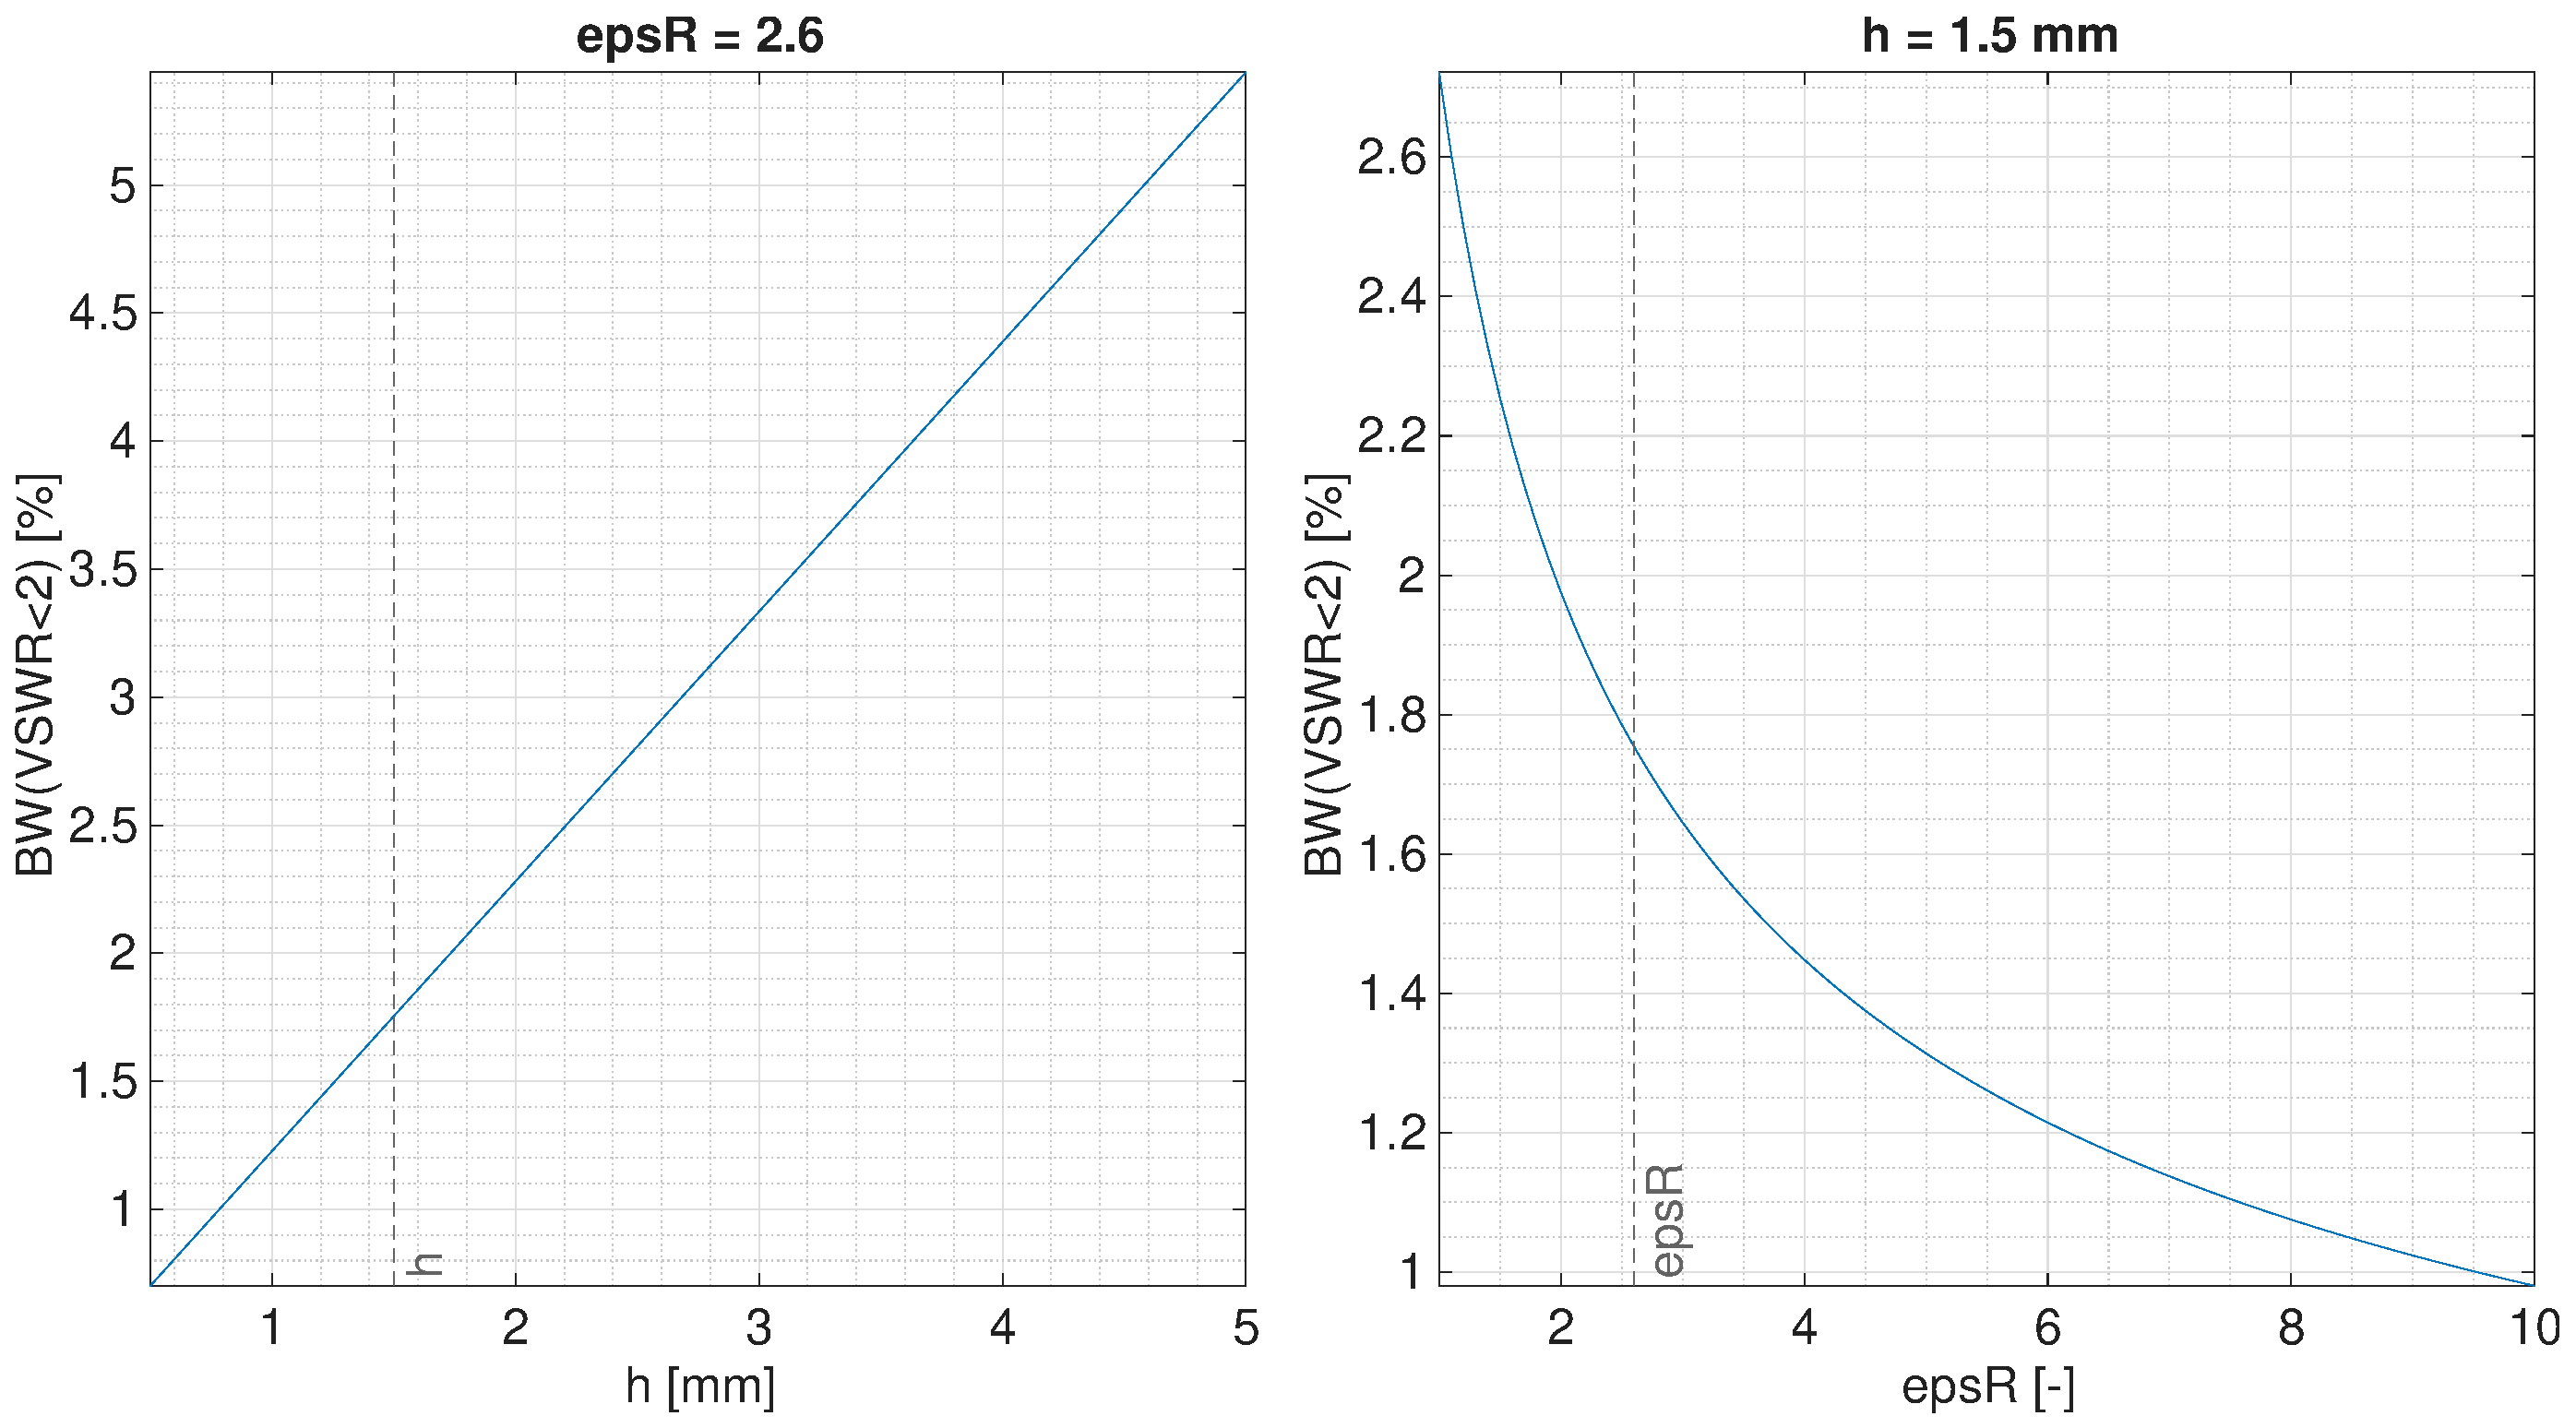
\includegraphics[width=\textwidth]{src/bandwidth-material-dependence.eps}
                \caption{\label{fig:bandwidth-material-dependence}Dependence of the impedance bandwidth on substrate properties}
            \end{figure}

        \subsection{Radiation patterns}
            The computed antenna dimensions can be directly utilized to compute the radiation field patterns. The field pattern in the E-plane ($\varphi = 0$) is given by
            \begin{align}
                \label{eq:field-pattern-e-plane}
                F_E(\theta) &= \frac{\sin\(\dfrac{k_0h}{2}\cos(\theta)\)}{\dfrac{k_0h}{2}\cos(\theta)}\cos\(\dfrac{k_0L_{\mathrm{eff}}}{2}\sin(\theta)\),
            \end{align}
            where
            \begin{align}
                L_{\mathrm{eff}} &= \frac{c}{2f_{\mathrm{res}}\sqrt{\epsilon_{\mathrm{eff}}}}
            \end{align}
            is the effective half-wavelength (effective length of the patch $L+2\Delta L$), and the field pattern in the H-plane ($\varphi = \pi/2$) is given by
            \begin{align}
                \label{eq:field-pattern-h-plane}
                F_H(\theta) &= \cos(\theta)\frac{\sin\(\dfrac{k_0h}{2}\cos(\theta)\)}{\dfrac{k_0h}{2}\cos(\theta)}\frac{\sin\(\dfrac{k_0W}{2}\sin(\theta)\)}{\dfrac{k_0W}{2}\sin(\theta)}.
            \end{align}
            The resulting field patterns computed using Equations~\ref{eq:field-pattern-e-plane}~and~\ref{eq:field-pattern-h-plane} are shown in Figure~\ref{fig:field-patterns}.
            \begin{figure}[!ht]
                \centering
                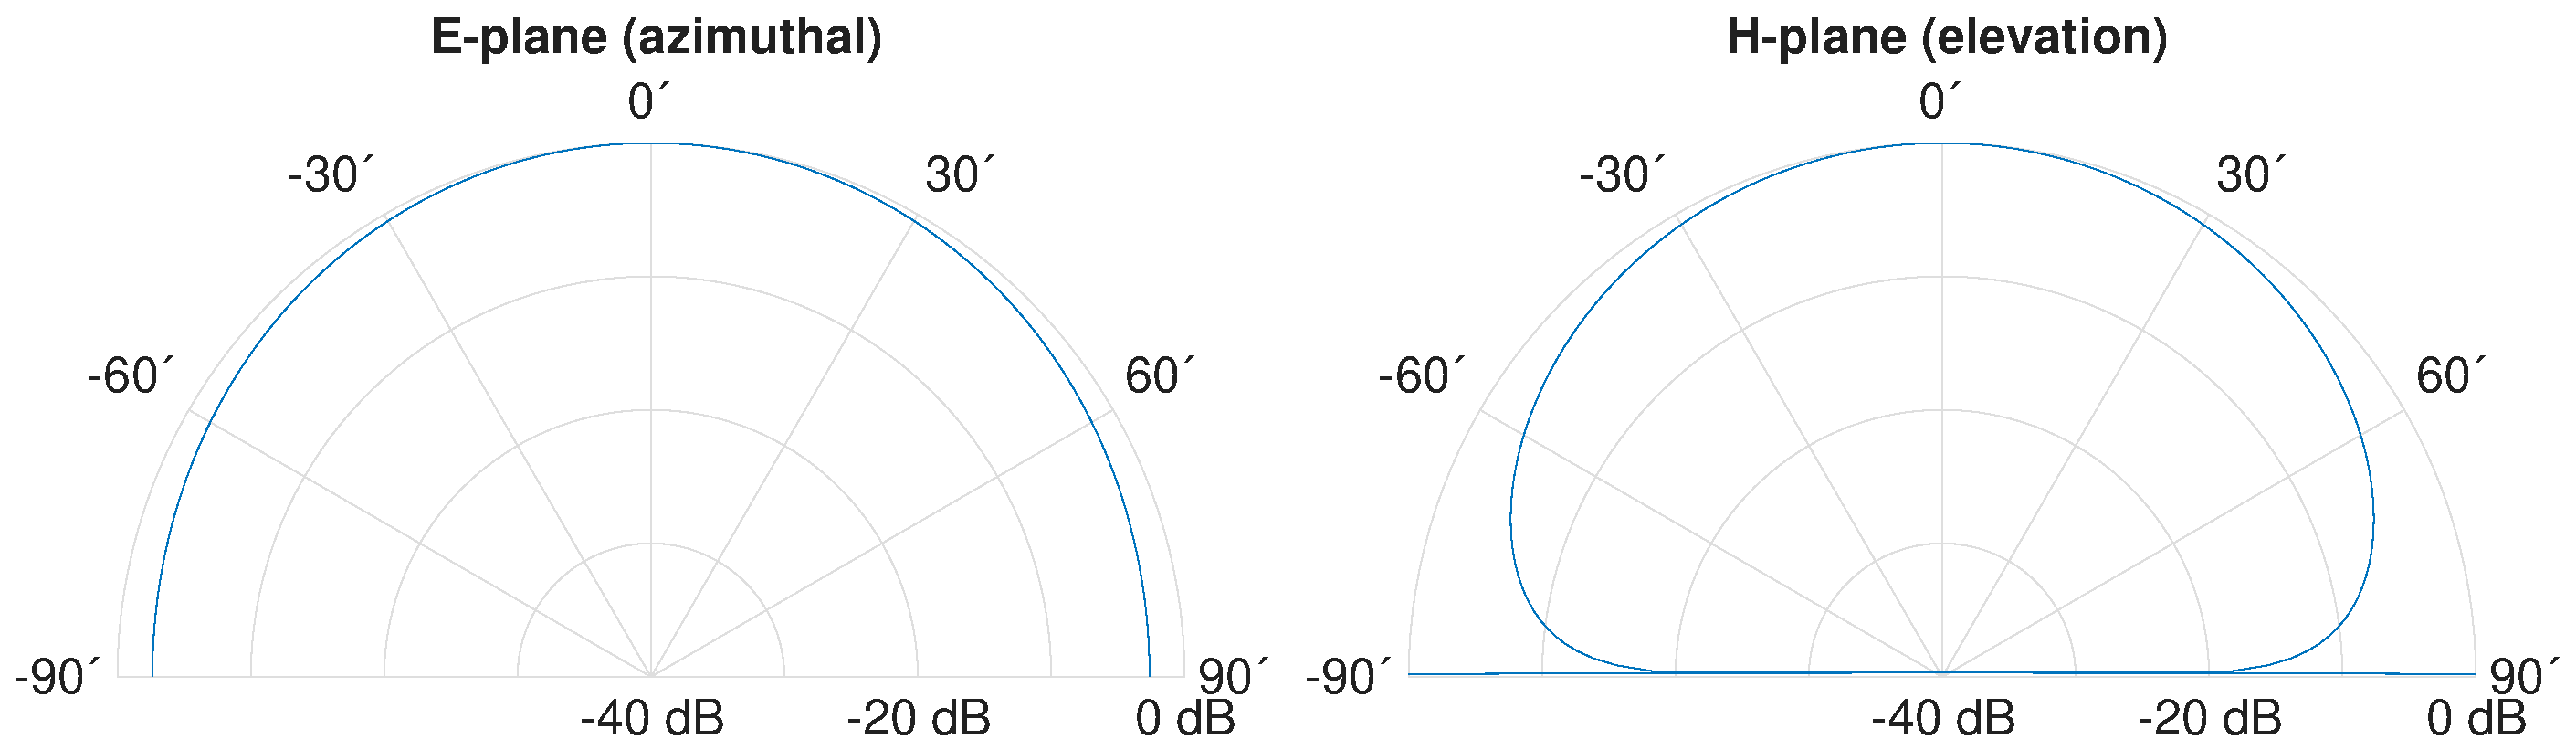
\includegraphics[width=\textwidth]{src/field-patterns.eps}
                \caption{\label{fig:field-patterns}Normalized field patterns}
            \end{figure}

    % \newpage
    \section{Measurement of a patch antenna}
        In the following section, measurement data are compared with the data obtained from the TLM computations. The models are created anew for the parameters of the measured antenna which are as follows:
        \begin{itemize}
            \item substrate height $h = 5\, \mathrm{mm}$,
            \item substrate material air ($\epsilon_r = 1$, $\tan(\delta) \approx 0$),
            \item patch length $L = 58\, \mathrm{mm}$,
            \item patch width $W = 61\, \mathrm{mm}$.
        \end{itemize}

        \subsection{Comparison of the measured data with transmission line models}
            \paragraph{Measurement 1.} The first measurement involves the fabricated antenna with the feed offset of $L_1 = 4\, \mathrm{mm}$. The comparison of the measured data with the TLM in terms the input impedance and the reflection coefficient is illustrated in Figure~\ref{fig:measurement1}.

            \paragraph{Measurement 2.} The second measurement involves the fabricated antenna with the feed offset of $L_1 = 16\, \mathrm{mm}$ which should be closest to optimal match out of the three. The comparison of the measured data with the TLM in terms the input impedance and the reflection coefficient is illustrated in Figure~\ref{fig:measurement2}.

            \paragraph{Measurement 3.} The third measurement involves the fabricated antenna with the feed offset of $L_1 = 28\, \mathrm{mm}$. The comparison of the measured data with the TLM in terms the input impedance and the reflection coefficient is illustrated in Figure~\ref{fig:measurement3}.

            \begin{figure}[!ht]
            \centering
                \begin{subfigure}{.8\textwidth}
                    \centering
                    \includegraphics[width=\textwidth]{src/measurement1.eps}
                    \caption{\label{fig:measurement1}Measurement 1: feed offset $4\, \mathrm{mm}$}
                \end{subfigure}\\[.5cm]
                \begin{subfigure}{.8\textwidth}
                    \centering
                    \includegraphics[width=\textwidth]{src/measurement2.eps}
                    \caption{\label{fig:measurement2}Measurement 2: feed offset $16\, \mathrm{mm}$}
                \end{subfigure}\\[.5cm]
                \begin{subfigure}{.8\textwidth}
                    \centering
                    \includegraphics[width=\textwidth]{src/measurement3.eps}
                    \caption{\label{fig:measurement3}Measurement 3: feed offset $28\, \mathrm{mm}$}
                \end{subfigure}
                \caption{\label{fig:measurements}Input impedance and reflection coefficient for different feed offsets}
            \end{figure}

        \subsection{Comparison of the measured and modelled resonant properties}
            From the comparison of the measured and modelled reflection coefficients shown in Figure~\ref{fig:measurements}, we can see that the resonant frequencies and impedance bandwidths are not the same. More specifically in the case of the best-matched antenna (Figure~\ref{fig:measurement2}), we can determine the resonant frequencies%
                \footnote{$f_{\mathrm{res}} = \min_{f \in (2\, \mathrm{GHz}, 3\, \mathrm{GHz})}|\Gamma(f)|$}
            as $f_{\mathrm{meas}} = 2.24\, \mathrm{GHz}$ in the case of the measured data and $f_{\mathrm{TLM}} = 2.29\, \mathrm{GHz}$ for the transmission line model. Furthermore, we can determine the impedance bandwidth of $\mathit{VSWR} < 2$ as $\mathit{BW}_{\mathrm{meas}} = 1.32\, \%$ in the case of the measured data and $\mathit{BW}_{\mathrm{TLM}} = 2.06\, \%$ for the transmission line model.

        \subsection{Discussion of differences}
            As we can see from the results, the properties of the measured and modelled antennas can slightly differ. These differences can be attributed to various simplifications and assumptions introduced during the analysis using the transmission line model. The main structural aspects which are simplified or neglected in the TLM are listed in the following summary:
            \begin{itemize}
                \item \emph{Substrate properties:} As opposed to reality, the TLM model assumes a perfectly homogeneous dielectric substrate with uniform properties.
                \item \emph{Finite ground plane:} The TLM assumes an infinite ground plane which is an unrealistic assumption for real fabrication.
                \item \emph{Radiation losses:} The inevitable radiation losses of the microstrip transmission line are neglected in the TLM.
                \item \emph{Fringing fields:} During the TLM analysis, the effects of the fringing fields around the edges of the patch are neglected.
                \item \emph{Fabrication possibilities}: The TLM assumes perfect geometrical dimension with zero tolerance.
                \item \emph{Higher-order modes:} The TLM neglects the propagation of higher-order modes.
            \end{itemize}

\end{document}
